\documentclass[Lecture.tex]{subfiles}
\begin{document}
\section{1.5: Exponential Functions}
\begin{frame}{Definition}
  \begin{defn}
    \begin{itemize}
    \item<1->
      A function $P(t)$ is {\it exponential with base a} if $P(t) = P_0a^t$.
    \item<2->
      The value $P_0$ is the {\it initial value}, $P_0 = P(0)$.
    \item<3->
      When $1 < a$, we say that $P$ models {\it exponential growth} and when $0 < a < 1$, we say that $P$ models {\it exponential decay}.
    \item<4->
      The base $a$ is sometimes called the {\it growth/decay factor}.
    \end{itemize}
  \end{defn}
\end{frame}

\begin{frame}{Relative Change}
  Let $P(t) = P_0a^t$.
  \onslide<2->{The relative change, $r$, of $P$ is given by}
  \begin{eqnarray*}
    \onslide<2->{r &=& \frac{P(t + 1) - P(t)}{P(t)}\\}
    \onslide<3->{&=& \frac{P_0a^{t + 1} - P_0a^t}{P_0a^t}\\}
    \onslide<4->{&=& \frac{P_0a^t\cdot a - P_0a^t}{P_0a^t}\\}
    \onslide<5->{&=& \frac{P_0a^t(a - 1)}{P_0a^t}\\}
    \onslide<6->{&=& a - 1.}
  \end{eqnarray*}
  \onslide<7->{\begin{rmk}
    \onslide<7->{Exponential functions have constant {\bf relative} change.}
    \onslide<8->{Linear functions have constant {\bf rate} of change.}
  \end{rmk}}
\end{frame}

\begin{frame}{Example}
  The body eliminates $40\%$ of the drug ampicillan (an antibiotic) each hour.
  \onslide<2->{Given a dose of $250$ mg, find a function, $Q(t)$, that models the quantity of the drug in the body $t$ hours after it has been administered.}
  \begin{itemize}
  \item<3->
    $Q_0 = Q(0) = 250$,
  \item<4->
    $Q(1) = 250(6/10) = 250(3/5)$,
  \item<5->
    $Q(2) = [250(3/5)](3/5) = 250(3/5)^2$,\\
    \onslide<6->{
      %\begin{center}
      $\vdots$}
    %\end{center}}
  \item<7->
    $Q(t) = [250(3/5)^{t - 1}](3/5) = 250(3/5)^t$.
  \end{itemize}
\end{frame}

\begin{frame}{Example}
  In 1995, there were 14 wolves reintroduced to Wyoming.
  \onslide<2->{By 2012 (17 years later), there were 207 wolves.}
  \onslide<3->{Assuming the growth of the population is exponential, find a function $P(t)$ modeling the population size as a function of $t$ years after 1995.}
  \begin{eqnarray*}
    \onslide<4->{P(17) &=& P(0)\cdot a^{17} = 14a^{17} = 207\\}
    \onslide<5->{\Rightarrow a^{17} &=& \frac{207}{14}\\}
    \onslide<6->{\Rightarrow a &=& \sqrt[17]{\frac{207}{14}} \approx 1.172}
  \end{eqnarray*}
  \onslide<7->{Therefore, 
    $$P(t) = 14\left(\frac{207}{14}\right)^{\frac{t}{17}} \approx 14(1.172)^t.$$}
\end{frame}

\begin{frame}{Example}
  Assume that $Q(t)$ is an exponential function.
  \onslide<2->{Suppose that $Q(20) = 88.2$ and $Q(23) = 91.4$.}
  \onslide<3->{
    \begin{enumerate}[(a)]
    \item
      Find the base.
      \begin{eqnarray*}
        \onslide<4->{\frac{91.4}{88.2} &=& \frac{Q(23)}{Q(20)}} \onslide<5->{= \frac{Q_0a^{23}}{Q_0a^{20}}} \onslide<6->{= a^{3}\\}
        \onslide<7->{\Rightarrow a &=& \sqrt[3]{\frac{91.4}{88.2}} \approx 1.012}
      \end{eqnarray*}
    \item
      Find the relative growth rate.
      $$\onslide<8->{r = a - 1} \onslide<9->{= \sqrt[3]{\frac{91.4}{88.2}} - 1 \approx 0.012}$$
  \end{enumerate}
  }
\end{frame}

\begin{frame}{Graphs of Exponential Functions}
  \noindent
  \begin{multicols}{2}
    \begin{center}
      $1 < a$:
      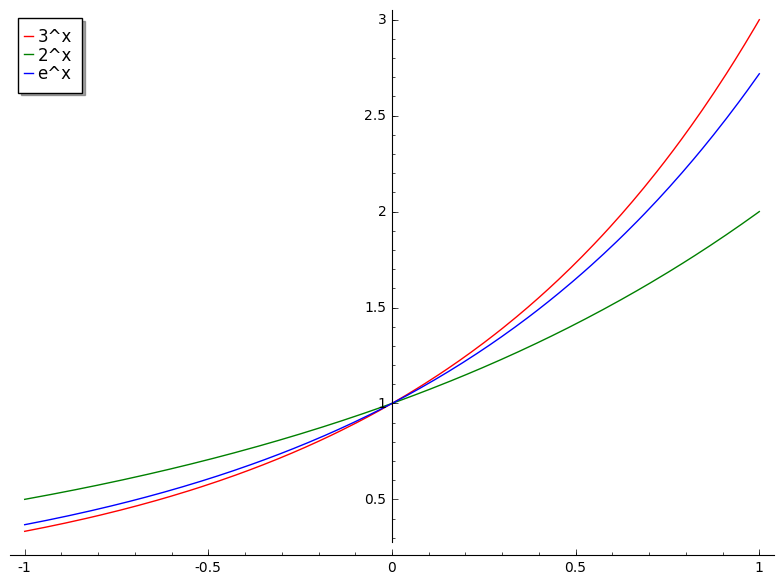
\includegraphics[scale=0.25]{exponentials1}
    \end{center}
    \columnbreak
    \begin{center}
      $0 < a < 1$:
      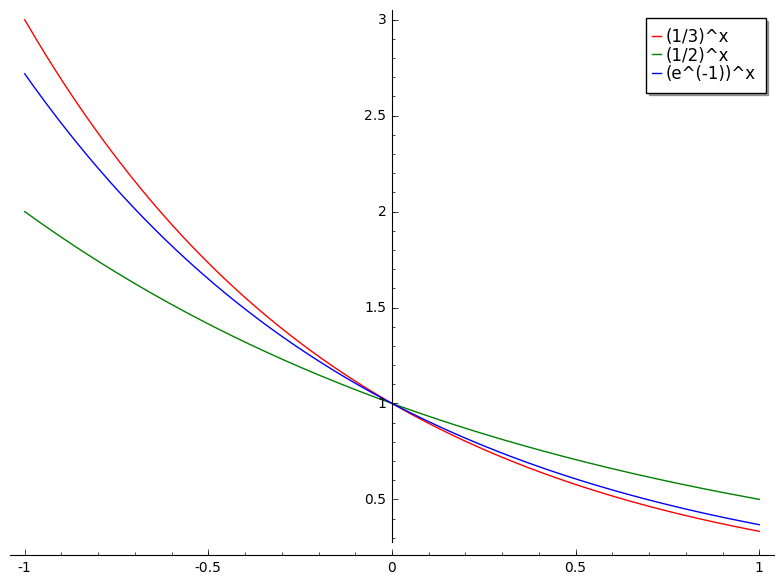
\includegraphics[scale=0.25]{exponentials2}
    \end{center}
  \end{multicols}
\end{frame}

\end{document}
